%%
%% This is file `gabarit-these-classique.tex',
%% generated with the docstrip utility.
%%
%% The original source files were:
%%
%% hecthese.dtx  (with options: `gabarit,phd,classique,francais')
%% 
%% This is a stripped version of the original file.
%% 
%% Copyright 2017-2019 HEC Montreal
%% 
%% This work may be distributed and/or modified under the
%% conditions of the LaTeX Project Public License, either version 1.3c
%% of this license or (at your option) any later version.
%% 
%% The latest version of this license is in
%% http://www.latex-project.org/lppl.txt
%% and version 1.3c or later is part of all distributions of LaTeX
%% version 2008/05/04 or later.
%% 
%% This work has the LPPL maintenance status `maintained'.
%% 
%% The Current Maintainer of this work is Benoit Hamel
%% <benoit.2.hamel@hec.ca>.
%% 
%% This work consists of the files hecthese.dtx, hecthese-fr.ins,
%% hecthese-en.ins, hecthese.pdf, hecthese-en.pdf
%% and the derived files listed in the README file.
%% 
%% GABARIT POUR UNE THÈSE CLASSIQUE
%%
%% Ceci est le fichier maître dans lequel vous inscrivez les métadonnées
%% relatives à votre travail, vous créez vos commandes et environnements
%% personnalisés, et à partir duquel vous lancez vos compilations.
%%
%% NE RÉDIGEZ PAS VOTRE THÈSE OU MÉMOIRE DANS CE FICHIER!
%%
%% Consultez la documentation de la classe hecthese pour de plus amples
%% informations.
%%
%% DÉCLARATION DE LA CLASSE DE DOCUMENT
%%
%% La classe est déclarée avec le type de document et les langues par
%% défaut. Inscrivez dans la liste d'options la taille de police de
%% caractères (10pt, 11pt, 12pt) ou laissez la classe charger la taille
%% par défaut : 12pt.
\documentclass[phdclassique,english,frenchb]{hecthese}
%%
%% PACKAGES À CHARGER
%%
%% Ajoutez tous les packages nécessaires à la rédaction de votre travail.
%% Consultez la documentation de la classe pour connaître la liste des
%% packages qui sont chargés par défaut. Assurez-vous cependant de suivre
%% les consignes suivantes :
%%
%% 1) Le package hyperref doit être chargé EN DERNIER si vous voulez qu'il
%% fonctionne correctement.
%% 2) Le package geometry est INCOMPATIBLE avec la classe memoir. Vous ne
%% devez pas l'utiliser dans votre travail. Consultez la documentation
%% de la classe memoir pour de plus amples informations.
%%
%% CHOIX D'UNE POLICE DE CARACTÈRES
%%
%% Choisissez le package mathptmx si vous voulez utiliser une police de type
%% Times, avec empattements, et le package mathpazo si vous voulez utiliser
%% une police de type Arial, sans empattements. Choisissez-en une et supprimez
%% l'autre, ou mettez-la en commentaires.
\usepackage{mathptmx}
%% \usepackage{mathpazo}

\usepackage{hyperref}
%%
%% PRODUCTION DE L'INDEX
%%
\makeindex
%%
%% STYLE BIBLIOGRAPHIQUE
%%
%% On utilise par défaut le style bibliographique francais issu du package
%% francais-bst. L'utilisation de ce style n'est pas obligatoire. Consultez
%% la documentation pour connaître la liste des styles compatibles avec la
%% langue de rédaction de votre thèse ou mémoire.
%%
\bibliographystyle{francais}
%%
%% MISE EN FORME DE LA TABLE DES MATIÈRES
%%
%% On inclut dans la table des matières toutes les divisions de document
%% jusqu'aux sous-sections. Si vous désirez avoir une table des matières
%% plus détaillée, indiquez dans les deux commandes ci-dessous jusqu'à
%% quel niveau vous voulez voir répertoriés dans la TDM.
%%
\setsecnumdepth{subsection} % Numérotation des sous-sections / Subsection numbering
\settocdepth{subsection} % Inclusion des sous-sections dans la TDM / Including subsections in the TOC
%%
%% MÉTADONNÉES DU DOCUMENT
%%
%% Le titre de votre travail. Si le titre est long, utilisez la commande \\
%% pour le mettre sur plusieurs lignes.
\HECtitre{Titre de la thèse ou du mémoire}
%% Le sous-titre de votre travail. S'il ne comporte pas de sous-titre, videz
%% le contenu des accolades.
\HECsoustitre{Sous-titre de la thèse}
%% L'auteur, c'est vous...
\HECauteur{Prénom Nom}
%% Nom de l'option de votre grade
\HECoption{Nom de l'option}
%% Mois du dépôt final de votre travail
\HECmoisDepot{Mai}
%% Année du dépôt final de votre travail
\HECanneeDepot{2017}
%% Le nom complet du président rapporteur et son genre (M ou F)
\HECpresidentRapporteur{Prénom Nom}{M ou F}
%% Le nom complet de votre directeur de recherche et son genre (M ou F)
\HECdirecteurRecherche{Prénom Nom}{M ou F}
%% Le nom complet de votre codirecteur de recherche et son genre (M ou F)
\HECcodirecteurRecherche{Prénom Nom}{M ou F}
%% L'université de provenance de votre codirecteur de recherche
\HECuniversiteCodirecteur{HEC Montréal}
%% Le nom complet du membre du jury
\HECmembreJury{Prénom Nom}
%% L'université de provenance du membre du jury
\HECuniversiteMembreJury{HEC Montréal}
%% Le nom complet de l'examinateur externe et son genre (M ou F)
\HECexaminateurExterne{Prénom Nom}{M ou F}
%% L'université de provenance de l'examinateur externe
\HECuniversiteExaminateur{HEC Montréal}
%% Le nom complet du représentant du directeur et son genre (M ou F)
\HECrepresentantDirecteur{Prénom Nom}{M ou F}
%%
%% OPTIONS DES PACKAGES CHARGÉS
%%
%% Si vos packages ont des options spécifiques à charger avant le début
%% du document, inscrivez-les ci-dessous. Si vous voulez outrepasser les
%% options des packages chargés par défaut avec la classe hecthese,
%% consultez la documentation pour en connaître la procédure.
%%
%% Options du package hyperref (inclure les métadonnées pdf dans les options) /
%% hyperref package option (including pdf metadata)
\hypersetup{%
colorlinks=true,
allcolors=black,
pdfauthor=\HECpdfauteur,
pdftitle=\HECpdftitre
}
%% Options de babel / babel options
\frenchbsetup{% 
og=«, fg=» % caractères « et » sont les guillemets
}
%%
%% DÉBUT DE LA THÈSE OU DU MÉMOIRE
%%
\begin{document}

%% Pages liminaires / frontmatter
\frontmatter

%% Page de garde / cover page
\mbox{}
\thispagestyle{empty}
\cleardoublepage

%% Page de titre
 \HECpagestitre


%% Résumé français / french abstract
 %% Fichier contenant le résumé français, les mots-clés et les méthodes de recherche.
\chapter*{Résumé}
\phantomsection\addcontentsline{toc}{chapter}{Résumé}
\thispagestyle{empty} % Première page non paginée / Unnumbered first page

%% Rédigez votre résumé français ici (350 à 500 mots).

\section*{Mots-clés}

%% Inscrivez vos mots-clés ici (15 maximum, incluant les méthodes de recherche ci-dessous).

\section*{Méthodes de recherche}

%% Inscrivez vos méthodes de recherche ici.

%% THÈSES ET MÉMOIRES PAR ARTICLES SEULEMENT
%% Si vous avez inséré des citations dans cette section, retirez les signes
%% de commentaires (%%) devant la commande ci-dessous et inscrivez le style
%% bibliographique et le nom du fichier .bib utilisés pour vos références.
%% \HECreferences{style}{nom-du-fichier-file-name}


%% Résumé anglais / english abstract
 %% Fichier contenant le résumé anglais, les mots-clés et les méthodes de recherche.
\chapter*{Abstract}
\phantomsection\addcontentsline{toc}{chapter}{Abstract}

%% Rédigez votre résumé anglais ici (350 à 500 mots).

\section*{Keywords}

%% Inscrivez vos mots-clés en anglais ici (15 maximum, incluant les méthodes de recherche ci-dessous).

\section*{Research methods}

%% Inscrivez vos méthodes de recherche en anglais ici.

%% THÈSES ET MÉMOIRES PAR ARTICLES SEULEMENT
%% Si vous avez inséré des citations dans cette section, retirez les signes
%% de commentaires (%%) devant la commande ci-dessous et inscrivez le style
%% bibliographique et le nom du fichier .bib utilisés pour vos références.
%% \HECreferences{style}{nom-du-fichier-file-name}


%% Table des matières (* pour ne pas inclure la TDM dans la TDM) /
%% Table of contents (* for excluding the TOC from the TOC)
\tableofcontents*
\cleardoublepage

%% Liste des tableaux / list of table
\listoftables
\cleardoublepage

%% Liste des figures / list of figures
\listoffigures
\cleardoublepage

%% Liste des abréviations / acronyms list
 %% Fichier contenant la liste des abréviations. Vous retrouverez ci-dessous un exemple
%% de liste. L'environnement HECabreviations prend en argument la plus longue des
%% abréviations. À la compilation, une liste en deux colonnes alignées est générée.
\chapter*{\HECtdmAbreviations}
\phantomsection\addcontentsline{toc}{chapter}{\HECtdmAbreviations}

\begin{HECabreviations}{ABBR}
\item[ABBR] Abréviation
\item[BAA] Baccalauréat en administration des affaires
\item[DESS] Diplôme d'études supérieures spécialisées
\item[HEC] Hautes études commerciales
\item[MBA] Maîtrise en administration des affaires
\item[MSc] Maîtrise
\item[PhD] Doctorat
\end{HECabreviations}


%% Dédicace / dedication
 %% Fichier contenant la dédicace
%% N'inscrivez rien entre les accolades de la commande \chapter*{},
%% sauf si vous voulez voir la dédicace dans la table des matières.

\chapter*{}

\begin{HECdedicace}
%% Rédigez votre dédicace ici.
\end{HECdedicace}


%% Remerciements / acknowledgements
 %% Fichier contenant les remerciements
\chapter*{\HECtdmRemerciements}
\phantomsection\addcontentsline{toc}{chapter}{\HECtdmRemerciements}

%% Rédigez vos remerciements ici.


%% Avant-propos / preface
 %% Fichier contenant l'avant-propos
\chapter*{\HECtdmAvantPropos}
\phantomsection\addcontentsline{toc}{chapter}{\HECtdmAvantPropos}

%% Rédigez votre avant-propos ici.

%% THÈSES ET MÉMOIRES PAR ARTICLES SEULEMENT
%% Si vous avez inséré des citations dans cette section, retirez les signes
%% de commentaires (%%) devant la commande ci-dessous et inscrivez le style
%% bibliographique et le nom du fichier .bib utilisés pour vos références.
%% \HECreferences{style}{nom-du-fichier-file-name}


%% Partie principale de la thèse ou du mémoire / mainmatter
\mainmatter

%% Introduction
\chapter{Introduction}
This is a template for writing a thesis according to the Technion specifications. 
Please, however, check with the graduate school website to see if any specifications have changed. 
This template was written by Boaz Shuval (January 2019). 

\section{Instructions}

This template is provided as is. Please check with the Technion graduate school website to see if the guidelines have changed, as they often do. For
the latest directions from the graduate school, see: 
\url{https://graduate.technion.ac.il/graduation/thesis-editing/}
(This is the website address circa January 2019). 

All files use UTF-8 encoding. Make sure your LaTeX system supports this encoding. 

\subsection{Preparing the Thesis}

\begin{enumerate}
\item The main.tex file is the main file to be compiled. Place it (with the other thesis files) in the same directory as the \verb".cls" and \verb".sty"
    files provided.                                                                                                                                          
    \item  The main class is \verb"technionThesis.cls."
   It has the the following options:  
   \begin{itemize}
       \item  hyperref       ---  Add hyperlinks
       \item  publist        ---  Add a list of publications in the front pages (update list in thesissetup.sty)
       \item  addack         ---  Add an acknowledgments page (only for final version!)
       \item  advisement     ---  Use "advisement" instead of "supervision" in front pages (a pet peeve of mine)
       \item  spacepar       ---  Add a blank line between paragraphs
       \item  firstparindent ---  Indent the first paragraph of a chapter/section
       \item  libertine      ---  Use a different selection of fonts, based on libertine, for the English part of the thesis. (See note 4)
    \end{itemize}
\item In the file \verb"technionThesisSetup.sty" you must input your details in the various commands. It is pretty self explanatory. 
\item The class loads a number of packages that the class author (Boaz Shuval) uses regularly. It also sets up theorem-style environments.
   If you know what you're doing, feel free to change things as you see fit. Otherwise, leave this alone. 
   \begin{enumerate}
       \item Environments are defined using amsthm. The following environments are available:
           \begin{itemize}
               \item Theorem-style: theorem, lemma, corollary, proposition, conjecture
      (Heading in bold, text in italics)
      These all share consecutive numbering, in the format (chapter.number)
  \item Definition-style: definition, example, assumption, condition 
      (Heading in bold, text upright)
      These are numbered (chapter.number) with their own numbering. Assumption and condition have alphanumeric numbering (A,B,C, etc.)
  \item Remark-style: remark, question, discussion
      (Heading in italics, text upright)
      These are numbered (chapter.number) with their own numbering. Discussion is unnumbered. 
  \item Proof environments: proof, IEEEproof. Both have a black square at the proof end. 
    \end{itemize}
\item  Packages loaded (partial listing):
    \begin{itemize}
        \item mathtools (which loads amsmath)
        \item amsthm, amssymb
        \item IEEEtrantools (loads IEEEeqnarray, and also sets the bibliography style)
        \item graphicx 
        \item tikz (including various useful tikz libraries) 
        \item cleveref (for referring to sections, etc, using \verb"\Cref", automagically adding the header)
        \item stackrel
        \item accents  (for adding symbols above symbols)
        \item xspace (for adding a smart space after a macro command)
        \item tabto  (add a tabstop for lining things up)
        \item algorithm2e (ruled, vlined)
        \item url
        \item polyglossia (for Hebrew support)
        \item longtable (for a table that runs over more than one page; useful for the abstract)
        \item booktabs, multirow (for nicer tables)
    \end{itemize}
    \end{enumerate}
\item Place all of your own commands in the file \verb"Example/technionThesisMacros.sty". That is, various \verb"\newcommand" and \verb"\DeclareMathOperator" are defined here. I've defined a few
   useful ones for you to get started. 
\item There are now \verb".tex" files for you to edit: 
    \begin{itemize}
        \item \verb"abstract.tex"         for your abstract in English (200-500 words)
        \item \verb"habstract.tex"        for your abstract in Hebrew (500-2000 words)
        \item \verb"acknowledgments.tex"  for your acknowledgments in English
        \item \verb"hacknowledgments.tex" for your acknowledgments in Hebrew
        \item \verb"introduction.tex"     for your introduction chapter
        \item \verb"chapfirst.tex"        for your first chapter 
        \item \verb"chapsecond.tex"       for your second chapter (add additional chapters as you see fit)
        \item \verb"discussion.tex"       for your discussion/conclusions chapter
        \item \verb"appendix.tex"         for your appendix (appendices must appear in their own chapters, and not as part of the main text). 
   \end{itemize}
   \end{enumerate}

   \subsection{Compilation}
Compile using xelatex. If you are using latexmk, you may include in the compilation directory a file called \verb".latexmkrc"
with the following line: 

\verb"$pdflatex = 'xelatex --shell-escape %O %S';"

This tells latexmk to use xelatex for compilation, so you need not worry
about this.
You may also compile this on overleaf (again, use xelatex). 

The Hebrew portion of the thesis is based on the polyglossia package. It uses the David CLM font for Hebrew. Thus, you must install the culmus fonts
for this to work on your installation. 

\subsection{ Be a pal}
Please share this template with your friends and colleagues. 
If you enjoyed using it, consider sending me a note to let me know. 
If you find a bug, or have asuggestion for improvement, I'd love to know about it.

\section{Files in this Template}

\begin{itemize}
    \item  \verb"technionThesis.cls"     ---  The class file
    \item  \verb"technionThesisSetup.sty"        ---  Setup data fields
    \item  \verb"README.md"                
    \item  Inside the Example directory:
        \begin{itemize}
    \item  \verb"abbrev.tex"               
    \item  \verb"abstract.tex"             
    \item  \verb"acknowledgments.tex"
    \item  \verb"appendix.tex"
    \item  \verb"chapfirst.tex"
    \item  \verb"chapsecond.tex"
    \item  \verb"discussion.tex"
    \item  \verb"habstract.tex"          ---  Hebrew abstract
    \item  \verb"hacknowledgments.tex"   ---  Hebrew acknowledgments
    \item  \verb"introduction.tex"
    \item  \verb"main.tex"               ---  Main thesis file
    \item  \verb"mybib.bib"
    \item  \verb"technionThesisMacros.sty"           ---  Define your macros here
\end{itemize}
\end{itemize}

\section{License}
This template is licensed under Creative Commons CC BY 4.0. 

\section{Notes}
\begin{enumerate}
    \item This template was tested on a mac running macOS 10.13, with TEXLIVE2017. It was also tested on overleaf in January 2019, which also runs TEXLIVE2017. 
    \item There is a bug when using TEXLIVE2018, which manifests itself in the figure/table numbering. If you encounter this bug, use the memoir package from
          TEXLIVE2017, instead. 
    \item The template uses the Memoir package internally. The chapter heading design is a modified version of a design by Vincent Zoonekynd 
        (it is modified from the BlueBox style in \url{https://ctan.org/pkg/memoirchapterstyles}).  
       \item If using the libertine option, make sure to use the latest version of newtxmath, available from \url{https://ctan.org/pkg/newtx}
   (download the file \verb"newtxmath.sty" to the home directory)
   \end{enumerate}


   \section{ Version History}
31 January 2019:    Version 1.0




\section{A Section} 
The remainder of this file is a boilerplate example
Equations are also fine: 
\[ 
    f(x) = x+2,
\] 
as are numbered equations:
\begin{equation}\label{eq:numbered int}
    g(y) = y.
\end{equation}
Of course, one may refer to a numbered equation such as~\eqref{eq:numbered int}. 

\section{Second section}
In this section we have a figure. 

\begin{figure}[t]
    \begin{center}
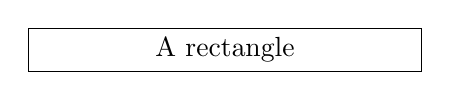
\begin{tikzpicture}
    \node[draw, minimum width = 5cm] {A rectangle};
\end{tikzpicture}
\end{center}
\caption[Short caption]{A very long caption for this figure. It is deliberately very long to illustrate the usefulness of the short caption for the table of figures. }
\label{fig:rectangle}
\end{figure}
\lipsum[10-13]


















%% Chapitres de développement / chapters
\include{chapitre-1}
\include{chapitre-2}
%% Fichier contenant un chapitre du développement. La classe génère
%% trois fichiers de chapitres par défaut. Si vous en avez besoin
%% davantage, enregistrez ce fichier sous un autre nom et incluez
%% le nouveau fichier dans votre gabarit avec la commande \include.
\chapter{Titre du chapitre / Chapter title}
\thispagestyle{empty} % Première page non paginée / First page is unnumbered

%% Écrivez votre chapitre ici.


%% Conclusion
%% Fichier contenant la conclusion
\chapter*{\HECtitreConclusion}
\phantomsection\addcontentsline{toc}{chapter}{\HECtitreConclusion}
\thispagestyle{empty} % Première page non paginée / First page is unnumbered

%% Rédigez votre conclusion ici.

%% THÈSES ET MÉMOIRES PAR ARTICLES SEULEMENT
%% Si vous avez inséré des citations dans cette section, retirez les signes
%% de commentaires (%%) devant la commande ci-dessous et inscrivez le style
%% bibliographique et le nom du fichier .bib utilisés pour vos références.
%% \HECreferences{style}{nom-du-fichier-file-name}


%% Index analytique / analytical index
\printindex

%% BIBLIOGRAPHIE / BIBLIOGRAPHY
%% Inscrivez le nom de votre fichier .bib entre les accolades.
\bibliography{}

\backmatter

%% Retour à la pagination romaine / Back to roman page numbering
\pagenumbering{roman}

%% Annexes / appendices
\appendix
 %% Fichier contenant une annexe. La classe ne génère qu'un seul
%% fichier annexe.tex par défaut. Si vous en avez besoin davantage,
%% enregistrez ce fichier sous un autre nom et incluez-le dans votre
%% gabarit avec la commande \include.
%%
%% Pour que la bibliographie et la (les) annexe(s) soient paginées
%% correctement, c'est-à-dire en chiffres arabes pour la bibliographie
%% et en chiffres romains pour les annexes, ces dernières doivent être
%% placées après la commande \backmatter. Ce faisant, la numérotation
%% des annexes s'en trouve désactivée. Vous devrez donc numéroter
%% vos annexes manuellement à l'intérieur de la commande \chapter.
\chapter{Annexe A -- Titre de l'annexe}

%% Rédigez votre annexe ici.

%% THÈSES ET MÉMOIRES PAR ARTICLES SEULEMENT
%% Si vous avez inséré des citations dans cette section, retirez les signes
%% de commentaires (%%) devant la commande ci-dessous et inscrivez le style
%% bibliographique et le nom du fichier .bib utilisés pour vos références.
%% \HECreferences{style}{nom-du-fichier-file-name}


%% Page de garde de fin / back cover page
\mbox{}
\thispagestyle{empty}

\end{document}
\endinput
%%
%% End of file `gabarit-these-classique.tex'.
